%%%%%%%%%%%%%%%%%%%%%%%%%%%%%%%%%%%%%%%%%%%%%%%%%%%%%%%%%%%%
%%%%%%%%%%%%%%%%%%%%%%%%%%%%%%%%%%%%%%%%%%%%%%%%%%%%%%%%%%%%
\section{APIs and File Formats}
\label{implem:apis-and-file-formats}

Our primary goal is to improve interoperability between proving systems and frontend consumers of proving system implementations. We focused on two approaches for building standard interfaces for implementations:

\begin{enumerate}
\item We aim to develop a common API for proving systems to expose their capabilities to frontends in a way that is maximally agnostic to the underlying implementation details.
\item We aim to develop a file format for encoding a popular form of constraint systems (namely R1CS), and its assignments, so that proving system implementations and frontends can interact across language and API barriers.
\end{enumerate}

We did not aim to develop standards for interoperability between backends implementing the same (abstract) scheme, such as serialization formats for proofs (see the Extended Constraint-System Interoperability section for further discussion).


%%%%%%%%%%%%%%%%%%%%%%%%%%%%%%
\subsection{Generic API}

In order to help compare the performance and usability tradeoffs of proving system implementations, frontend application developers may wish to interact with the underlying proof systems via a generic interface, so that proving systems can be swapped out and the tradeoffs observed in practice. 
This also helps in an academic pursuit of analysis and comparison.

The abstract parties and objects in a NIZK are %as follows:
depicted in \reffig{fig:abstract-parties-and-objects-in-NIZK}.



\begin{figure}[H]\def\tmpfigcap{Abstract parties and objects in a NIZK}
\begin{center}
\refstepcounter{figure}\label{fig:abstract-parties-and-objects-in-NIZK}%
\hypertarget{ht:figure:\thefigure}{}
\addcontentsline{lof}{figure}{Figure~\thefigure{}: \tmpfigcap}
{
\bookmarksetup{level=3,color=\colorbkmfig}
\bookmark[dest=ht:figure:\thefigure]{Figure~\thefigure}%
\internallinenumbers
{
\nolinenumbers
\def\figlang{\hyperlink{def:language}{\scalebox{.75}{Language}}}
\def\figgen{Gen}
\def\figpp{pp}
\def\figwitness{\hyperlink{def:witness}{Witness}}
\def\figinstance{\hyperlink{def:instance}{Instance}}
\def\figprover{Prover}
\def\figproof{Proof}
\def\svgwidth{.99\textwidth}
\input{figs/implem--api-diagram.pdf_tex}
}
}
%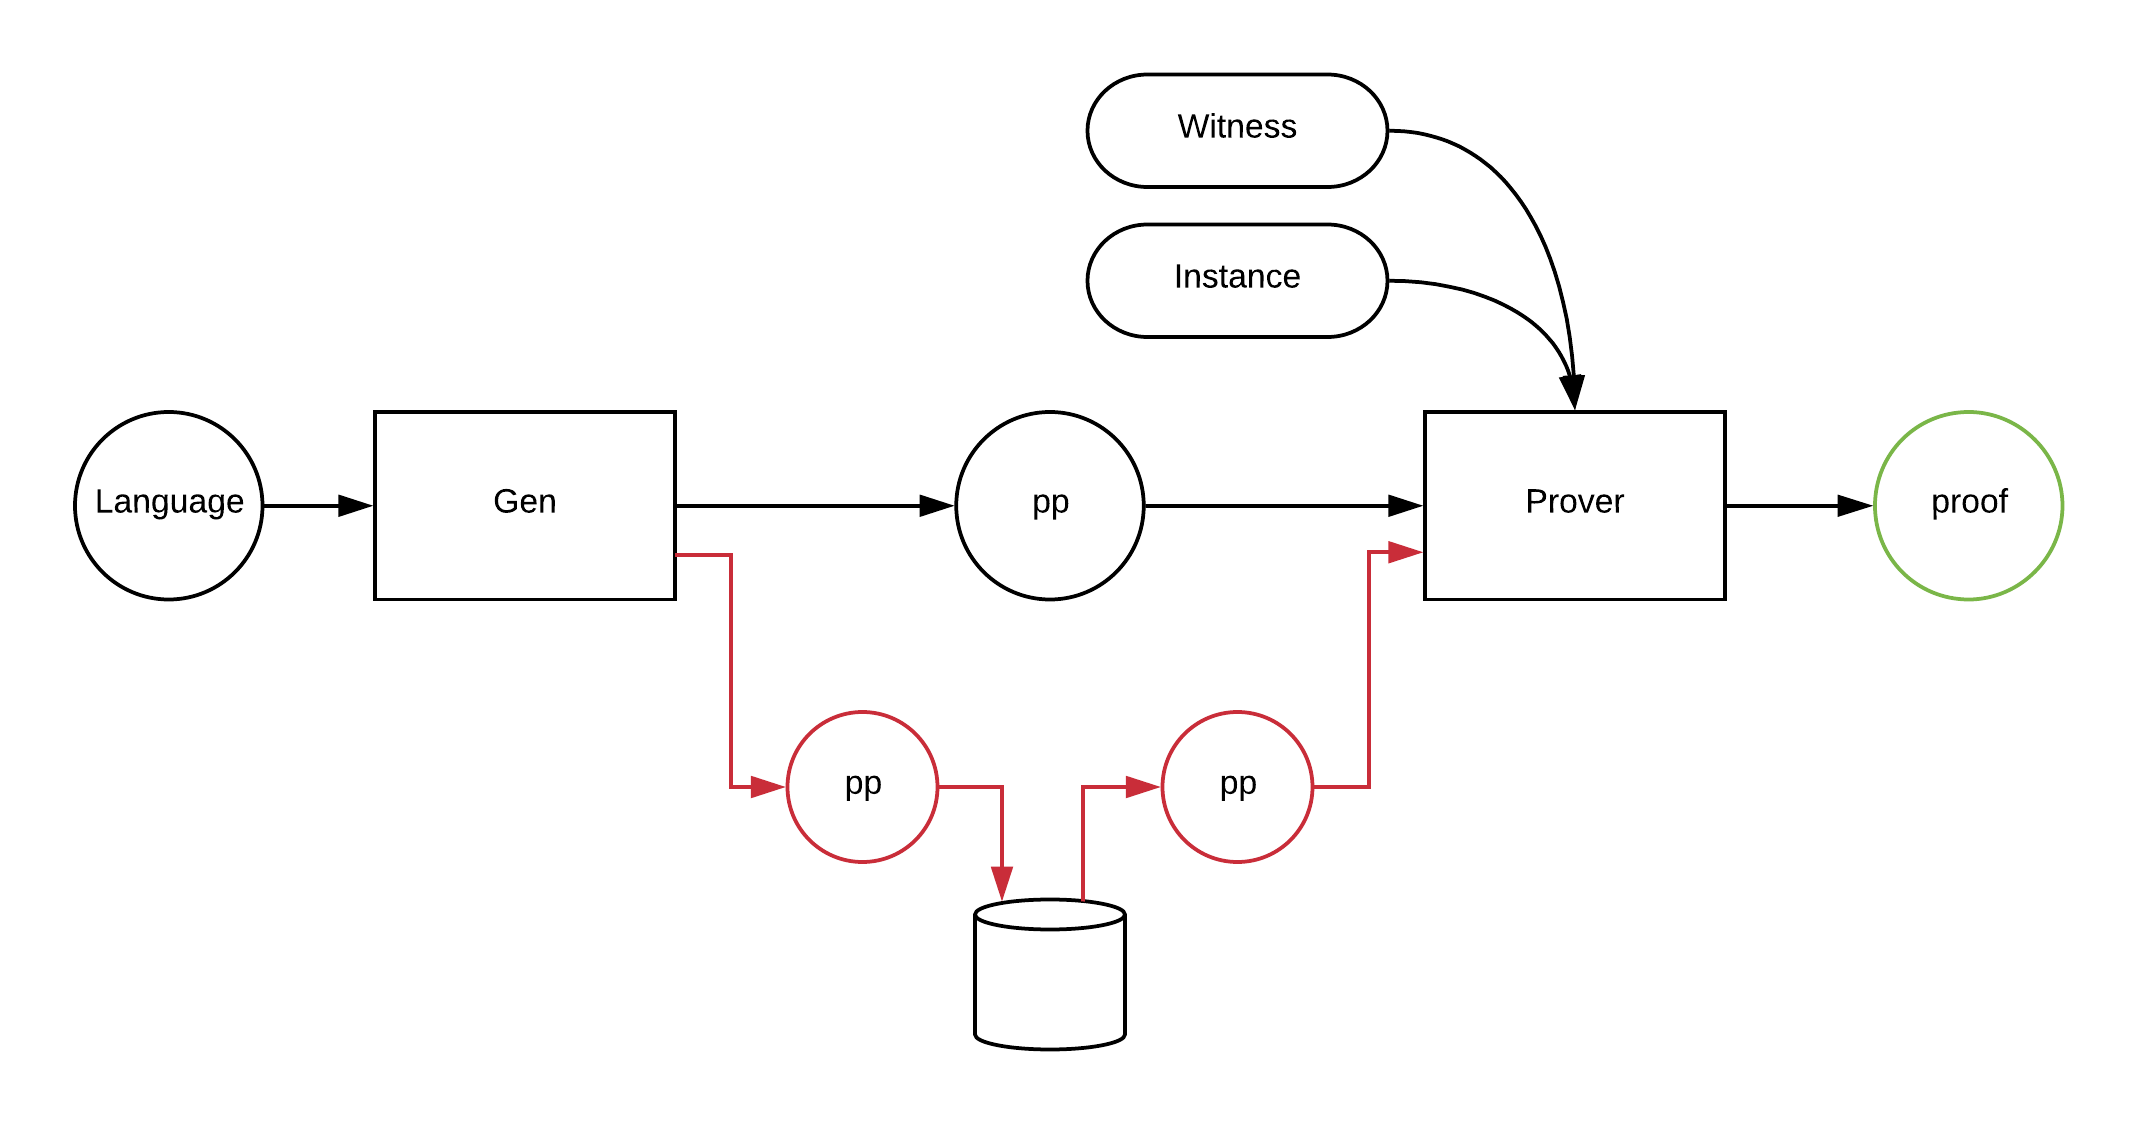
\includegraphics[width=\textwidth]{figs/implem--api-diagram.png}
\pdfcomment[author={Aur{\'e}lien Nicolas}]{the Verifier could appear here. \textCR\textCR PP, Instance, and Proof go into the Verifier box.}

{\centering \textbf{Figure \thefigure. }\tmpfigcap}
\end{center}
\end{figure}


We did not complete a generic API design for proving systems, but we did survey numerous tradeoffs and design approaches for such an API that may be of future value.

We separate the APIs and interfaces between the universal and non-universal NIZK setting. In the universal setting, the NIZK's CRS generation is independent of the relation (i.e., one CRS enables proving any NP statement). In the non-universal settings, the CRS generation depends on the relation (represented as a constraint system), and a given CRS enables proving the statements corresponding to any instance with respect to the specific relation.


\vspace{.5em}
\def\tmptabtitle{APIs and interfaces by types of universality and preprocessing}
{\mytabcap{\tmptabtitle}{\tmptabtitle}\label{tab:apps:APIS-and-interfaces-by-univ-and-preproc}}
\vspace{-1.5em}
\begin{longtable}{|>{\begmin{.30}}l<{\myendmini}|>{\begmin{.30}}l<{\myendmini}|>{\begmin{.30}}l|} %%%the last column ends with \rowend, which closes the minipage and adds \\
\hline 
	   & \textbf{Preprocessing} \\ (Generate has superpolylogarithmic runtime / output size as function of constraint system size)
		 & \textbf{Non-preprocessing} \\ (Generate runtime and output size is fast and CRS is at most polylogarithmic in constraint system size) \rowend
%%%%%%
\hline \textbf{Non-universal} \\ (Generate needs constraint system as input)
     & QAP-based \\ \cite{2013:SP:Pinocchio}, \cite{2013:Eurocrypt:quadratic-span-programs-and-succinct-NIZKs-without-PCPs}, \cite{2013:crypto:SNARKs-for-C}
		 & ? \rowend
%%%%%%
\hline {\textbf{Universal}} \\ (Generate needs just a size bound)
     & vnTinyRAM \\ vRAM \\ Bulletproofs (with explicit CRH)
		 & Bulletproofs (with PRG-based CRH generation) \rowend
%%%%%%
\hline \textbf{Universal and scalable}\\ (Generate needs nothing but security parameter)
		 & (impossible)
		 & ``Fully scalable'' SNARKs based on PCD (recursive composition) \rowend
\hline
\end{longtable}

In any case, we identified several capabilities that proving systems may need to express via a generic interface:

\begin{enumerate}
 \item The creation of CRS objects in the form of proving and verifying parameters, given the input language or size bound.
 \item The serialization of CRS objects into concrete encodings.
 \item Metadata about the proving system such as the size and characteristic of the field (for arithmetic constraints).
 \item Witness objects containing private inputs known only to the prover, and Instance objects containing public inputs known to the prover and verifier.
 \item The creation of Proof objects when supplied proving parameters, an Instance, and a Witness.
 \item The verification of Proof objects given verifying parameters and an Instance.
\end{enumerate}

\textbf{Future work:} 
We would like to see a concrete API design which leverages our tentative model, with additional work to encode concepts such as recursive composition and the batching of proving and verification operations.


%%%%%%%%%%%%%%%%%%%%%%%%%%%%%%
\subsection{R1CS File Format}

There are many frontends for constructing constraint systems, and many backends which consume constraint systems (and variable assignments) to create or verify proofs. We focused on creating a file format that frontends and backends can use to communicate constraint systems and variable assignments. Goals include simplicity, ease of implementation, compactness and avoiding hard-coded limits.

Our initial work focuses on R1CS due to its popularity and familiarity. 
Refer to the \hyperref[chap:security]{Security Track} document for more information about constraint systems. 
The design we arrived at is tentative and requires further iteration. 
Implementation and specification work will appear at \myurl{https://github.com/zkpstandard/file\_formats}.


\emph{R1CS (Rank 1 Constraint Systems)} is an NP-complete language for specifying relations as a system of bilinear constraints (i.e., a rank 1 quadratic constraint system), 
as defined in \cite[Appendix E in extended version]{2013:crypto:SNARKs-for-C}; %%%[BCGTV13, Appendix E in extended version]; 
this is a more intuitive reformulation of QAP \emph{QAP (Quadratic Arithmetic Program)}, 
defined in \cite{2013:SP:Pinocchio}. %%%[PHGR13]. 
R1CS is the native constraint system language of many ZK proof constructions (see the \hyperref[chap:security]{Security Track} document), including many ZK proof applications in operational deployment.

Our proposed format makes heavy use of variable-length integers which are prevalent in the (space-efficient) encoding of an R1CS. 
We refer to VarInt as a variable-length unsigned integer, and SignedVarInt as a variable-length signed integer. 
We typically use VarInt for lengths or version numbers, and SignedVarInt for field element constants. 
The actual description of a VarInt is not yet specified.

We’ll be working with primitive variable indices of the following form:

{\ttfamily
ConstantVar $\shortleftarrow$  SignedVarInt(0)\\
InstanceVar(i) $\shortleftarrow$  SignedVarInt(-(i + 1))\\
WitnessVar(i) $\shortleftarrow$  SignedVarInt(i + 1)\\
VariableIndex $\shortleftarrow$ ConstantVar / InstanceVar(i) / WitnessVar(i)
}

\emph{ConstantVar} represents an indexed constant in the field, usually assigned to one. 
\emph{InstanceVar} represents an indexed variable of the instance, or the public input, serialized with negative indices. 
\emph{WitnessVar} represents an indexed variable of the witness, or the private/auxiliary input, serialized with positive indices. 
\emph{VariableIndex} represents one of any of these possible variable indices.

We’ll also be working with primitive expressions of the following form:

{\ttfamily
Coefficient $\shortleftarrow$ SignedVarInt \\
Sequence(Entry) $\shortleftarrow$  | length: VarInt | length * Entry | \\
LinearCombination $\shortleftarrow$  Sequence(| VariableIndex | Coefficient |)
}
\begin{itemize}
    \item Coefficients must be non-zero.
    \item Entries should be sorted by type, then by index:
		\begin{itemize}
        \item | ConstantVar | sorted(InstanceVar) | sorted(WitnessVar) |
		\end{itemize}
\end{itemize}

{\ttfamily
Constraint $\shortleftarrow$  \\
| A: LinearCombination | B: LinearCombination | C: LinearCombination |
}

We represent a \emph{Coefficient} (a constant in a linear combination) with a \emph{SignedVarInt}. 
(TODO: there is no constraint on its canonical form.) These should never be zero. 
We express a \emph{LinearCombination} as sequences of \emph{VariableIndex} and \emph{Coefficient} pairs. 
Linear combinations should be sorted by type and then by index of the \emph{VariableIndex}; 
i.e., \emph{ConstantVar} should appear first, \emph{InstanceVar} should appear second (ascending) and \emph{WitnessVar} should appear last (ascending).

We express constraints as three \emph{LinearCombination} objects A, B, C, where the encoded constraint represents A * B = C.

The file format will contain a header with details about the constraint system that are important for the backend implementation or for parsing.

{\ttfamily
Header(version, vals) \shortleftarrow\\
| version: VarInt | vals: Sequence(SignedVarInt) |
}

The \emph{vals} component of the \emph{Header} will contain information such as:
\begin{itemize}
  \item  {\tt P} \shortleftarrow\ Field characteristic
  \item  {\tt D} \shortleftarrow\ Degree of extension
  \item  {\tt N\_X} \shortleftarrow\ Number of instance variables
  \item  {\tt N\_W} \shortleftarrow\ Number of witness variables
\end{itemize}

The representation of elements of extension fields is not currently specified, so {\tt D} should be 1.

The file format contains a magic byte sequence  “R1CSstmt”, a header, and a sequence of constraints, as follows:

{\ttfamily
R1CSFile \shortleftarrow\\
| "R1CSstmt" | Header(0, [ P, D, N\_X, N\_W, … ]) | Sequence(Constraint) |
}

Further values in the header are undefined in this specification for version 0, and should be ignored. The file extension “.r1cs” is used for R1CS circuits.

\textbf{Further work:} We wish to have a format for expressing the assignments for use by the backend in generating the proof. We reserve the magic “R1CSasig” and the file extention “.assignments” for this purpose. We also wish to have a format for expressing symbol tables for debugging. We reserve the magic “R1CSsymb” and the file extention “.r1cssym” for this purpose.

In the future we also wish to specify other kinds of constraint systems and languages that some proving systems can more naturally consume.

